\documentclass[11pt,english]{article}

%%%%%%%%%%%%%%%%%%%%%%%%%%%%%%%%%%%%%%%%%%%%%%%%%%%%%%%%%%%
% Packages
%%%%%%%%%%%%%%%%%%%%%%%%%%%%%%%%%%%%%%%%%%%%%%%%%%%%%%%%%%%

% paper size & margins
\usepackage{fullpage}
\usepackage[showframe=false,margin=1in]{geometry}
\parindent=0pt

% font management
\usepackage{relsize}
\usepackage[T1]{fontenc} % for properly hyphenating words with accented chars
\usepackage[latin1]{inputenc}
\usepackage{babel}

% math
\usepackage{amsmath, amsthm, amssymb}
\usepackage{textcomp}
\usepackage{stmaryrd}
\usepackage{upgreek}
\usepackage{bm}
\usepackage[linesnumbered,ruled,vlined]{algorithm2e}


% assorted
\usepackage{url}
\usepackage{breakurl}
\usepackage{xspace}
\usepackage{comment}
\usepackage{color}
\usepackage{afterpage}
\usepackage{tikz}

%%%%%%%%%%%%%%%%%%%%%%%%%%%%%%%%%%%%%%%%%%%%%%%%%%%%%%%%%%%
% Shortcuts
%%%%%%%%%%%%%%%%%%%%%%%%%%%%%%%%%%%%%%%%%%%%%%%%%%%%%%%%%%%
\newcommand{\hide}[1]{}
\DeclareMathOperator*{\argmin}{arg\,min}
\newtheorem{theorem}{Theorem}[section]
\newtheorem{corollary}{Corollary}[theorem]
\newtheorem{lemma}[theorem]{Lemma}

%%%%%%%%%%%%%%%%%%%%%%%%%%%%%%%%%%%%%%%%%%%%%%%%%%%%%%%%%%%
% Title / Author
%%%%%%%%%%%%%%%%%%%%%%%%%%%%%%%%%%%%%%%%%%%%%%%%%%%%%%%%%%%
\begin{document}

\title{CS7643: Deep Learning \\
Fall 2019\\ HW1 Solutions}
\author{James Hahn}
\maketitle


%%%%%%%%%%%%%%%%%%%%%%%%%%%%%%%%%%%%%%%%%%%%%%%%%%%%%%%%%%%
% Body
%%%%%%%%%%%%%%%%%%%%%%%%%%%%%%%%%%%%%%%%%%%%%%%%%%%%%%%%%%%

\section{Gradient Descent}

	1.\\
	$\argmin_w f(w^{(t)}) + \langle w-w^{(t)}, \nabla f(w^{(t)})\rangle + \frac{\lambda}{2}\lVert w-w^{(t)}\rVert^2 \\
	\implies \frac{\delta}{\delta w} = \nabla_{w}f(w^{(t)}) + \lambda(w - w^{(t)}) \\
	\implies \nabla_{w}f(w^{(t)}) + \lambda(w - w^{(t)}) = 0 \\
	\implies \lambda w = \lambda w^{(t)} - \nabla_{w}f(w^{(t)}) \\
	\implies w^* = w^{(t)} - \frac{1}{\lambda}\nabla_{w}f(w^{(t)}) \\$
	This tells us the gradient descent update rule helps find the solution to the true, underlying weights by approximating a function, rather than solving the optimization problem through direct differentiation. The relationship between $\lambda$ and $\eta$ is that $\frac{1}{\lambda} = \eta$. If we see $\lambda$ to be a regularization parameter, this could indicate the lower the $\lambda$ (regularization parameter), the higher the overall regularization on the weights. This occurs because a lower $\lambda$ produces higher $\frac{1}{\lambda}$, placing more weight on per-iteration weight differences, leading to a slower learning/approximation process for our weights.
	\pagebreak

	2.\\
	We want to show $\sum_{t=1}^{T}\langle w^{(t)} - w^*, v_t\rangle \leq \frac{||w^*||^2}{2\eta} + \frac{\eta}{2}\sum_{t=1}^{T}||v_t||^2$. As a preliminary step, let's simplify the problem. We will prove a lemma based on the update rule provided to us.
	
	\begin{lemma}
		$w^{(t+1)} = -\eta \sum_{i=1}^{t} v_t$\\
		We are given $w^{(1)} = 0$. For a proof by induction, the base case for $t=2$ is as follows: $w^{(2)} = w^{(1)} -\eta v_1 = -\eta v_1 = -\eta \sum_{i=1}^{1} v_t$, which is the trivial base case. For a non-trivial base case, such as $t=3$, we see the following: $w^{(3)} = w^{(2)} -\eta v_1 = -\eta v_1 -\eta v_2 = -\eta \sum_{i=1}^{2} v_t$. As such, we will show this follows for future $t$. Assume we have some $w^{(t+1)} = -\eta \sum_{i=1}^{t} v_t$. Now, $w^{(t+2)} = w^{(t+1)} - \eta v_{t+1} = -\eta \sum_{i=1}^{t} v_t - \eta v_{t+1} = -\eta [(\sum_{i=1}^{t} v_t) + v_{t+1}] = -\eta \sum_{i=1}^{t+1} v_t$. As such, the lemma holds. $\qed$
	\end{lemma}

	First, we decompose the LHS of the inequality. Namely, $\sum_{t=1}^{T} \langle\ w^{(t)} - w^*, v_t\rangle = \sum_{t=1}^{T} \langle\,w^{(t)}, v_t\rangle - \sum_{t=1}^{T} \langle\,w^*, v_t\rangle = \sum_{t=1}^{T} \langle\,w^{(t)}, v_t\rangle - \langle\,w^*, \sum_{t=1}^{T} v_t\rangle$.\\
	
	Second, by utilizing Lemma 1.1, we observe the following transformation of the first term on the RHS of the above equation:\\
	RHS first term = $\sum_{t=1}^{T} \langle\ w^{(t)} - w^*, v_t\rangle \\
	= \sum_{t=1}^{T} \langle\ -\eta \sum_{u=1}^{t-1} v_u, v_t\rangle \\
	= -\eta \sum_{t=1}^{T} \langle\ \sum_{u=1}^{t-1} v_u, v_t\rangle \\
	= -\eta (\frac{\langle \sum_{t=1}^{T} v_t, \sum_{t=1}^{T} v_t\rangle}{2} - \frac{\sum_{t=1}^{T} ||v_t||^2}{2})\\
	= -\frac{\eta}{2} ||\sum_{t=1}^{T} v_t||^2 + \frac{\eta}{2} \sum_{t=1}^{T} ||v_t||^2\\
	= -\frac{1}{2\eta} ||w^{(t+1)}||^2 + \frac{\eta}{2} \sum_{t=1}^{T} ||v_t||^2$\\

	Third, we simplify the second term on the RHS of the first equation with the use of Lemma 1.1:\\
	RHS second term = $\langle\,w^*, \sum_{t=1}^{T} v_t\rangle \\
	= \langle w^*, -\frac{1}{\eta} w^{(t+1)}\rangle \qquad (\text{from Lemma 1.1:} \thinspace\thinspace w^{(t+1)} = -\eta \sum_{i=1}^{t} v_t \implies \sum_{i=1}^{t} v_t = -\frac{1}{\eta} w^{(t+1)}) \\
	= -\frac{1}{\eta}\langle w^*, w^{(t+1)}\rangle$\\
	
	So, we have finally expanded the LHS of the inequality:\\
	LHS = $-\frac{1}{2\eta} ||w^{(t+1)}||^2 + \frac{\eta}{2} \sum_{t=1}^{T} ||v_t||^2 +\frac{1}{\eta}\langle w^*, w^{(t+1)}\rangle$ \\
	The key thing to note here is that $\frac{\eta}{2} \sum_{t=1}^{T} ||v_t||^2$ already appears on the given RHS of the inequality, so they cancel each other out. To simplify the problem and to further prove the inequality, all we need to show is $-\frac{1}{2\eta} ||w^{(t+1)}||^2 +\frac{1}{\eta}\langle w^*, w^{(t+1)}\rangle \leq \frac{||w^*||^2}{2\eta}$.\\
	
	First, we see $-\frac{1}{2\eta} ||w^{(t+1)}||^2$ is negative since it's the product of a negative fraction and a positive distance. Second, we see $\frac{1}{\eta}\langle w^*, w^{(t+1)}\rangle = \frac{1}{2\eta}\langle w^*, w^{(t+1)}\rangle + \frac{1}{2\eta}\langle w^*, w^{(t+1)}\rangle$. Third, $\langle w^*, w^{(t+1)}\rangle \leq \langle w^{(t+1)}, w^{(t+1)}\rangle = \|w^{(t+1)}\|^2$ and $\langle w^*, w^{(t+1)}\rangle \leq \langle w^{*}, w^{*}\rangle$. Therefore, with these observed properties, we know $-\frac{1}{2\eta}\| w^{(t+1)}\|^2 \leq - \frac{1}{2\eta}\langle w^*, w^{(t+1)}\rangle \implies -\frac{1}{2\eta}\| w^{(t+1)}\|^2 + \frac{1}{2\eta}\langle w^*, w^{(t+1)}\rangle \leq 0$. Additionally, $\frac{1}{2\eta}\langle w^*, w^{(t+1)}\rangle \leq \frac{1}{2\eta}\|w^*\|^2$. \\
	
	Finally, since we know $-\frac{1}{2\eta}\| w^{(t+1)}\|^2 + \frac{1}{2\eta}\langle w^*, w^{(t+1)}\rangle \leq 0$ and $\frac{1}{2\eta}\langle w^*, w^{(t+1)}\rangle \leq \frac{1}{2\eta}\|w^*\|^2$, we get the summation of a negative term and term that's less than the RHS of the inequality we're trying to prove, so we observe $-\frac{1}{2\eta} ||w^{(t+1)}||^2 +\frac{1}{\eta}\langle w^*, w^{(t+1)}\rangle \leq \frac{||w^*||^2}{2\eta}$. So, we have proved the simpler inequality we established above.\\
	
	$\therefore$ $\sum_{t=1}^{T}\langle w^{(t)} - w^*, v_t\rangle \leq \frac{||w^*||^2}{2\eta} + \frac{\eta}{2}\sum_{t=1}^{T}||v_t||^2 \qquad\qed$
	\pagebreak
	
	3.\\
	We must show for $\bar{w} = \frac{1}{T}\sum_{t=1}^{T} w^{(t)}$, we get $f(\bar{w}) - f(w^*) \leq \frac{1}{T}\sum_{t=1}^{T}\langle w^{(t)} - w^*, \nabla f(w^{(t)})\rangle$ . In the problem statement for question 1, we were told ``When $f$ is convex, this approximation forms a lower bound of $f$, referring to equation 2. As such, if we assume $f$ is convex, which is reasonable since $w^*$ minimizes $f$, we get\\
	$f(w^*) \geq f(w^{(t)}) + \langle w^* - w^{(t)}, \nabla f(w^{(t)})\rangle\\
	\implies f(w^*) - f(w^{(t)}) \geq \langle w^* - w^{(t)}, \nabla f(w^{(t)})\rangle \\
	\implies f(w^{(t)}) - f(w^*) \leq \langle w^{(t)} - w^*, \nabla f(w^{(t)})\rangle \\
	\implies \frac{1}{T}\sum_{t=1}^{T} \left[ f(w^{(t)}) - f(w^*) \right] \leq \frac{1}{T}\sum_{t=1}^{T} \langle w^{(t)} - w^*, \nabla f(w^{(t)})\rangle \\
	\implies \frac{1}{T}\sum_{t=1}^{T} [f(w^{(t)})] - f(w^*) \leq \frac{1}{T}\sum_{t=1}^{T} \langle w^{(t)} - w^*, \nabla f(w^{(t)})\rangle\\$
	The definition of convexity states if $f(x)$ is convex, then $f(tx) \leq tf(x)$ for some variable or function $t$. So, we know $f(\bar{w}) = f(\frac{1}{T}\sum_{t=1}^{T} w^{(t)}) \leq \frac{1}{T}\sum_{t=1}^{T} f(w^{(t)})$\\
	$\implies f(\bar{w}) - f(w^*) \leq \frac{1}{T}\sum_{t=1}^{T} \langle w^{(t)} - w^*, \nabla f(w^{(t)})\rangle$\\
	From question 2, we proved $\sum_{t=1}^{T}\langle w^{(t)} - w^*, v_t\rangle \leq \frac{||w^*||^2}{2\eta} + \frac{\eta}{2}\sum_{t=1}^{T}||v_t||^2$, so we get:\\
	$\implies f(\bar{w}) - f(w^*) \leq \frac{1}{T}\left[\frac{||w^*||^2}{2\eta} + \frac{\eta}{2}\sum_{t=1}^{T}||\nabla f(w^{(t)})||^2\right]\\
	\implies f(\bar{w}) - f(w^*) \leq \frac{||w^*||^2}{2T\eta} + \frac{\eta}{2T}\sum_{t=1}^{T}||\nabla f(w^{(t)})||^2$\\
	Now, if we just treat $B$ and $\rho$ as upper bounds for $\|w\|^2$ and $\|\nabla f(w^{(t)})\|$ respectively, as given in the problem, we get\\
	$\implies f(\bar{w}) - f(w^*) \leq \frac{B^2}{2T\eta} + \frac{\eta}{2T}\sum_{t=1}^{T}\rho^2\\
	\implies f(\bar{w}) - f(w^*) \leq \frac{B^2}{2T\eta} + \frac{\eta T\rho^2}{2T}$\\
	With simple algebra, the $T$ cancels out on the second term of the RHS, and we can substitute $\eta = \sqrt{\frac{B^2}{\rho^2 T}}$, which is given to us, into the equation:\\
	$\implies f(\bar{w}) - f(w^*) \leq \frac{B^2}{2T\sqrt{\frac{B^2}{\rho^2 T}}} + \frac{\sqrt{\frac{B^2}{\rho^2 T}}\rho^2}{2}\\
	\implies f(\bar{w}) - f(w^*) \leq \frac{B^2}{2T\frac{B}{\rho}\sqrt{\frac{1}{T}}} + \frac{\frac{B}{\rho}\rho^2\sqrt{\frac{1}{T}}}{2}\\
	\implies f(\bar{w}) - f(w^*) \leq \frac{B\rho}{2\sqrt{T}} + \frac{B\rho}{2\sqrt{T}}\\
	\implies f(\bar{w}) - f(w^*) \leq \frac{B\rho}{\sqrt{T}}$\\
	As shown above, the convergence rate of $w^*$ is $\mathcal{O}(\frac{1}{\sqrt{T}})$ i.e. upper bound of $f(\bar{w}) - f(w^*) \propto \frac{1}{\sqrt{T}}$. $\qquad \qed$
	\pagebreak
	
	4.\\
	No. We will show this with a simple counter-example. We were given $w^{(1)} = 0$ in this problem. Additionally, we are given the objective function $f(w) = \frac{1}{2}(w-2)^2 + \frac{1}{2}(w+1)^2$. We want to show the objective function does not always decrease after each iteration, assuming the gradient of the objective function at each iteration is randomly selected from the gradients of the two sub-terms of the objective function. As such, we either have $f'_1(w) = w-2$ or $f'_2(w) = w+1$ with equal probability. We use the update rule $w^{(t+1)} = w^{(t)} - \eta f'(w)$.
	
	First, we see $f(w^{(1)}) = \frac{1}{2}(0-2)^2 + \frac{1}{2}(0+1)^2 = 2 + 0.5 = 2.5$. So, we see the gradient is
	\[
	f'(w) =
	\begin{cases}
	-2 & \text{if $f'_1(w)$} \\
	1 & \text{if $f'_2(w)$} \\
	\end{cases}
	\]
	Let's use $f'_1(w)$ first. We see $w^{(2)}_1 = w^{(1)} - \eta f'_1(w) = 0 - \eta (-2) = 2\eta$. As such, $f(w^{(2)}_1) = \frac{1}{2}(2\eta-2)^2 + \frac{1}{2}(2\eta+1)^2 = \frac{1}{2}(4\eta^2-8\eta + 4) + \frac{1}{2}(4\eta^2 + 4\eta + 1) = 4\eta^2 - 4\eta + 5$. We know $\eta > 0$, as provided in the problem description, so all we can infer is the new loss function is less than 5, but we cannot assume it increased.
	
	Next, let's observe $f'_2(w)$. We see $w^{(2)}_2 = w^{(1)} - \eta f'_2(w) = 0 - \eta (1) = -\eta$. As such, $f(w^{(2)}_2) = \frac{1}{2}(-\eta-2)^2 + \frac{1}{2}(-\eta+1)^2 = \frac{1}{2}(\eta^2+4\eta+4) + \frac{1}{2}(\eta^2-2\eta+1) = \eta^2+\eta+2.5$. Since $\eta > 0$, we know for sure the new value of the objective function is greater than 2.5. Therefore, the value has increased. 
	
	$\therefore$ We cannot guarantee the loss function will decrease.
\pagebreak

\section{Automatic Differentiation}
	$5(a).$ \\
	
	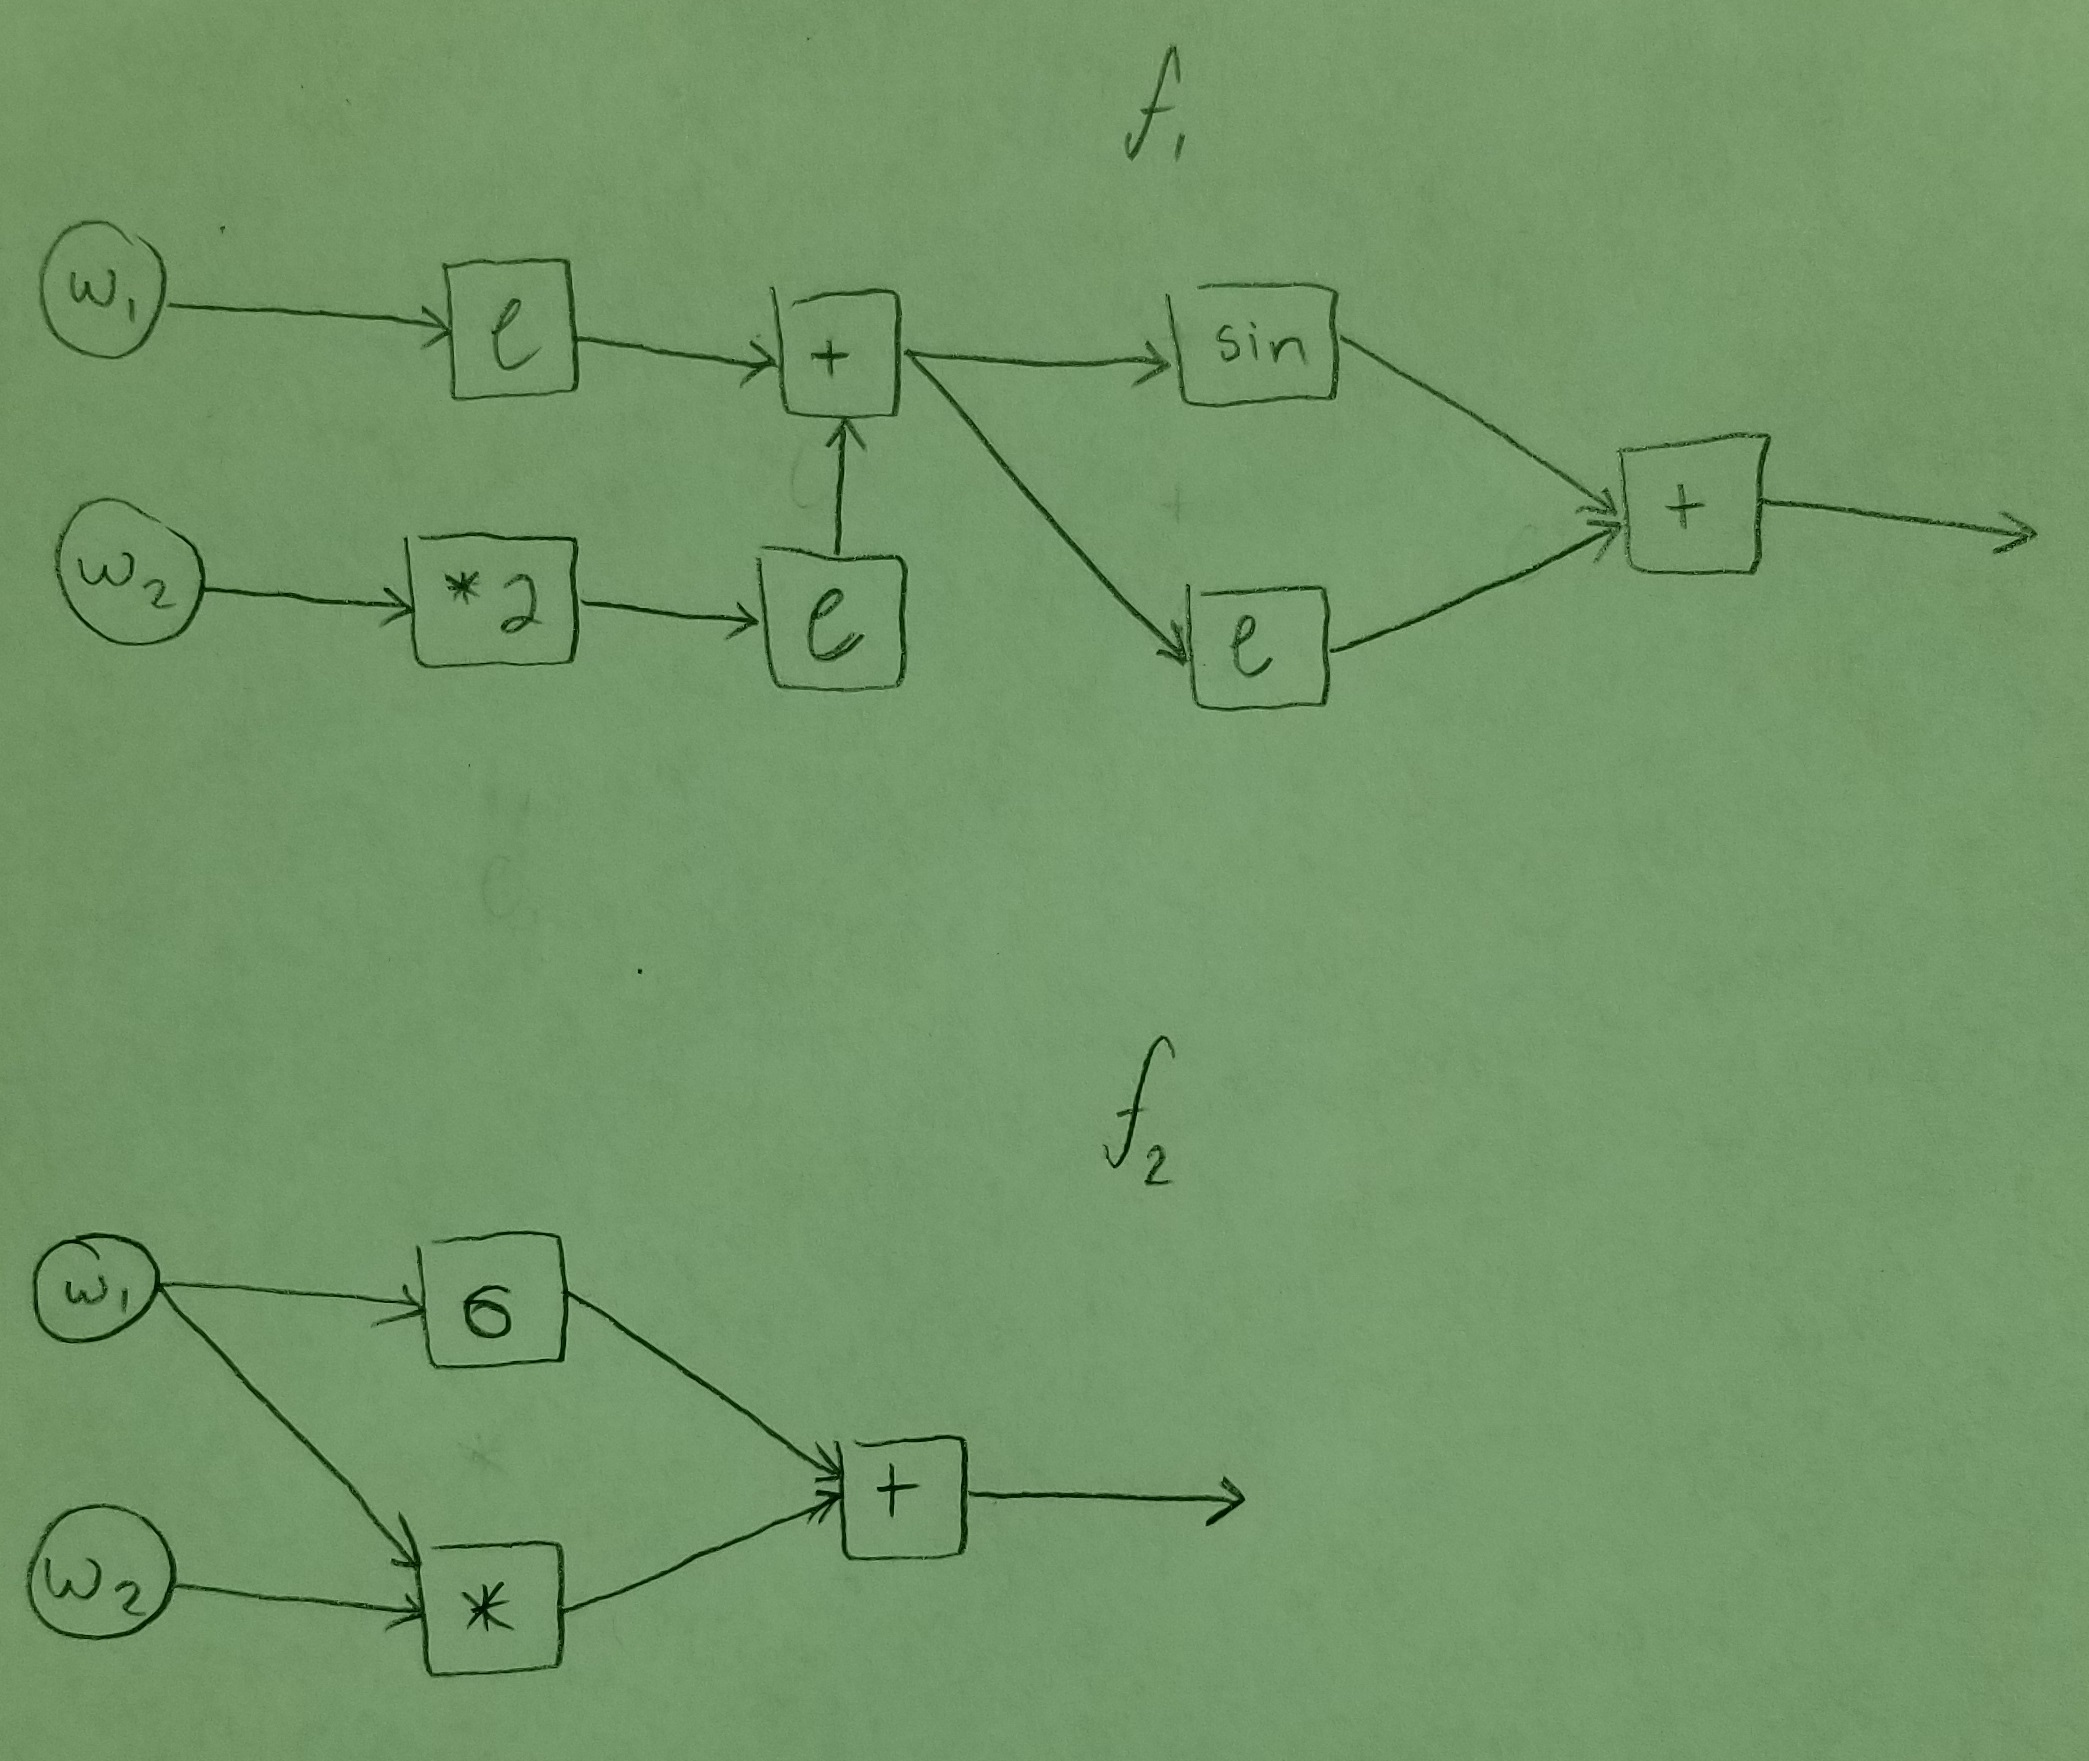
\includegraphics[scale=0.15]{5a.jpg}
	
	$f_1(w) = f_1(1, 2) = e^{e^{w_1} + e^{2w_2}} + sin(e^{w_1} + e^{2w_2}) = e^{e^{1} + e^{4}} + sin(e^{1} + e^{4}) = 7.8 \times 10^{24}$
	
	$f_2(w) = f_2(1, 2) = w_1w_2 + \sigma(w_1) = (1)(2) + \sigma(1) = 2 + \frac{1}{1+e^{-1}} = 2 + 0.731 = 2.731$\\
	\pagebreak
	
	$5(b).$\\
	
	$\frac{f_1(w_1 + 0.01, w_2) - f_1(w_1, w_2)}{0.01} = \frac{f_1(1.01, 2) - f_1(1, 2)}{0.01} = \frac{(8.018 \times 10^{24}) - (7.802 \times 10^{24})}{0.01} = \frac{2.162\times 10^{23}}{0.01} = 2.162\times 10^{25}$
	
	$\frac{f_1(w_1, w_2 + 0.01) - f_1(w_1, w_2)}{0.01} = \frac{f_1(1, 2.01) - f_1(1, 2)}{0.01} = \frac{(2.351\times 10^{25}) - (7.802 \times 10^{24})}{0.01} = \frac{1.571\times 10^{25}}{0.01} = 1.571\times 10^{27}$
	
	$\frac{f_2(w_1 + 0.01, w_2) - f_2(w_1, w_2)}{0.01} = \frac{f_2(1.01, 2) - f_2(1, 2)}{0.01} = \frac{2.753 - 2.731}{0.01} = \frac{0.022}{0.01} = 2.2$
	
	$\frac{f_2(w_1, w_2 + 0.01) - f_2(w_1, w_2)}{0.01} = \frac{f_2(1, 2.01) - f_2(1, 2)}{0.01} = \frac{2.741 - 2.731}{0.01} = \frac{0.01}{0.01} = 1$\\
	
	$J = \begin{bmatrix}
	2.162\times 10^{25} & 
	1.571\times 10^{27} \\[1ex] % <-- 1ex more space between rows of matrix
	2.2 & 
	1
	\end{bmatrix}$\\
	\pagebreak
	
	$\quad 5(c).$\\
	
	\includegraphics[scale=0.2]{5c.png}\\
	
	$J = \begin{bmatrix}
	2.120\times 10^{25} & 8.516\times 10^{26} \\
	2.197 & 1 \\[1ex] % <-- 1ex more space between rows of matrix
	\end{bmatrix}$\\
	\pagebreak
	
	$5(d).$\\
	
	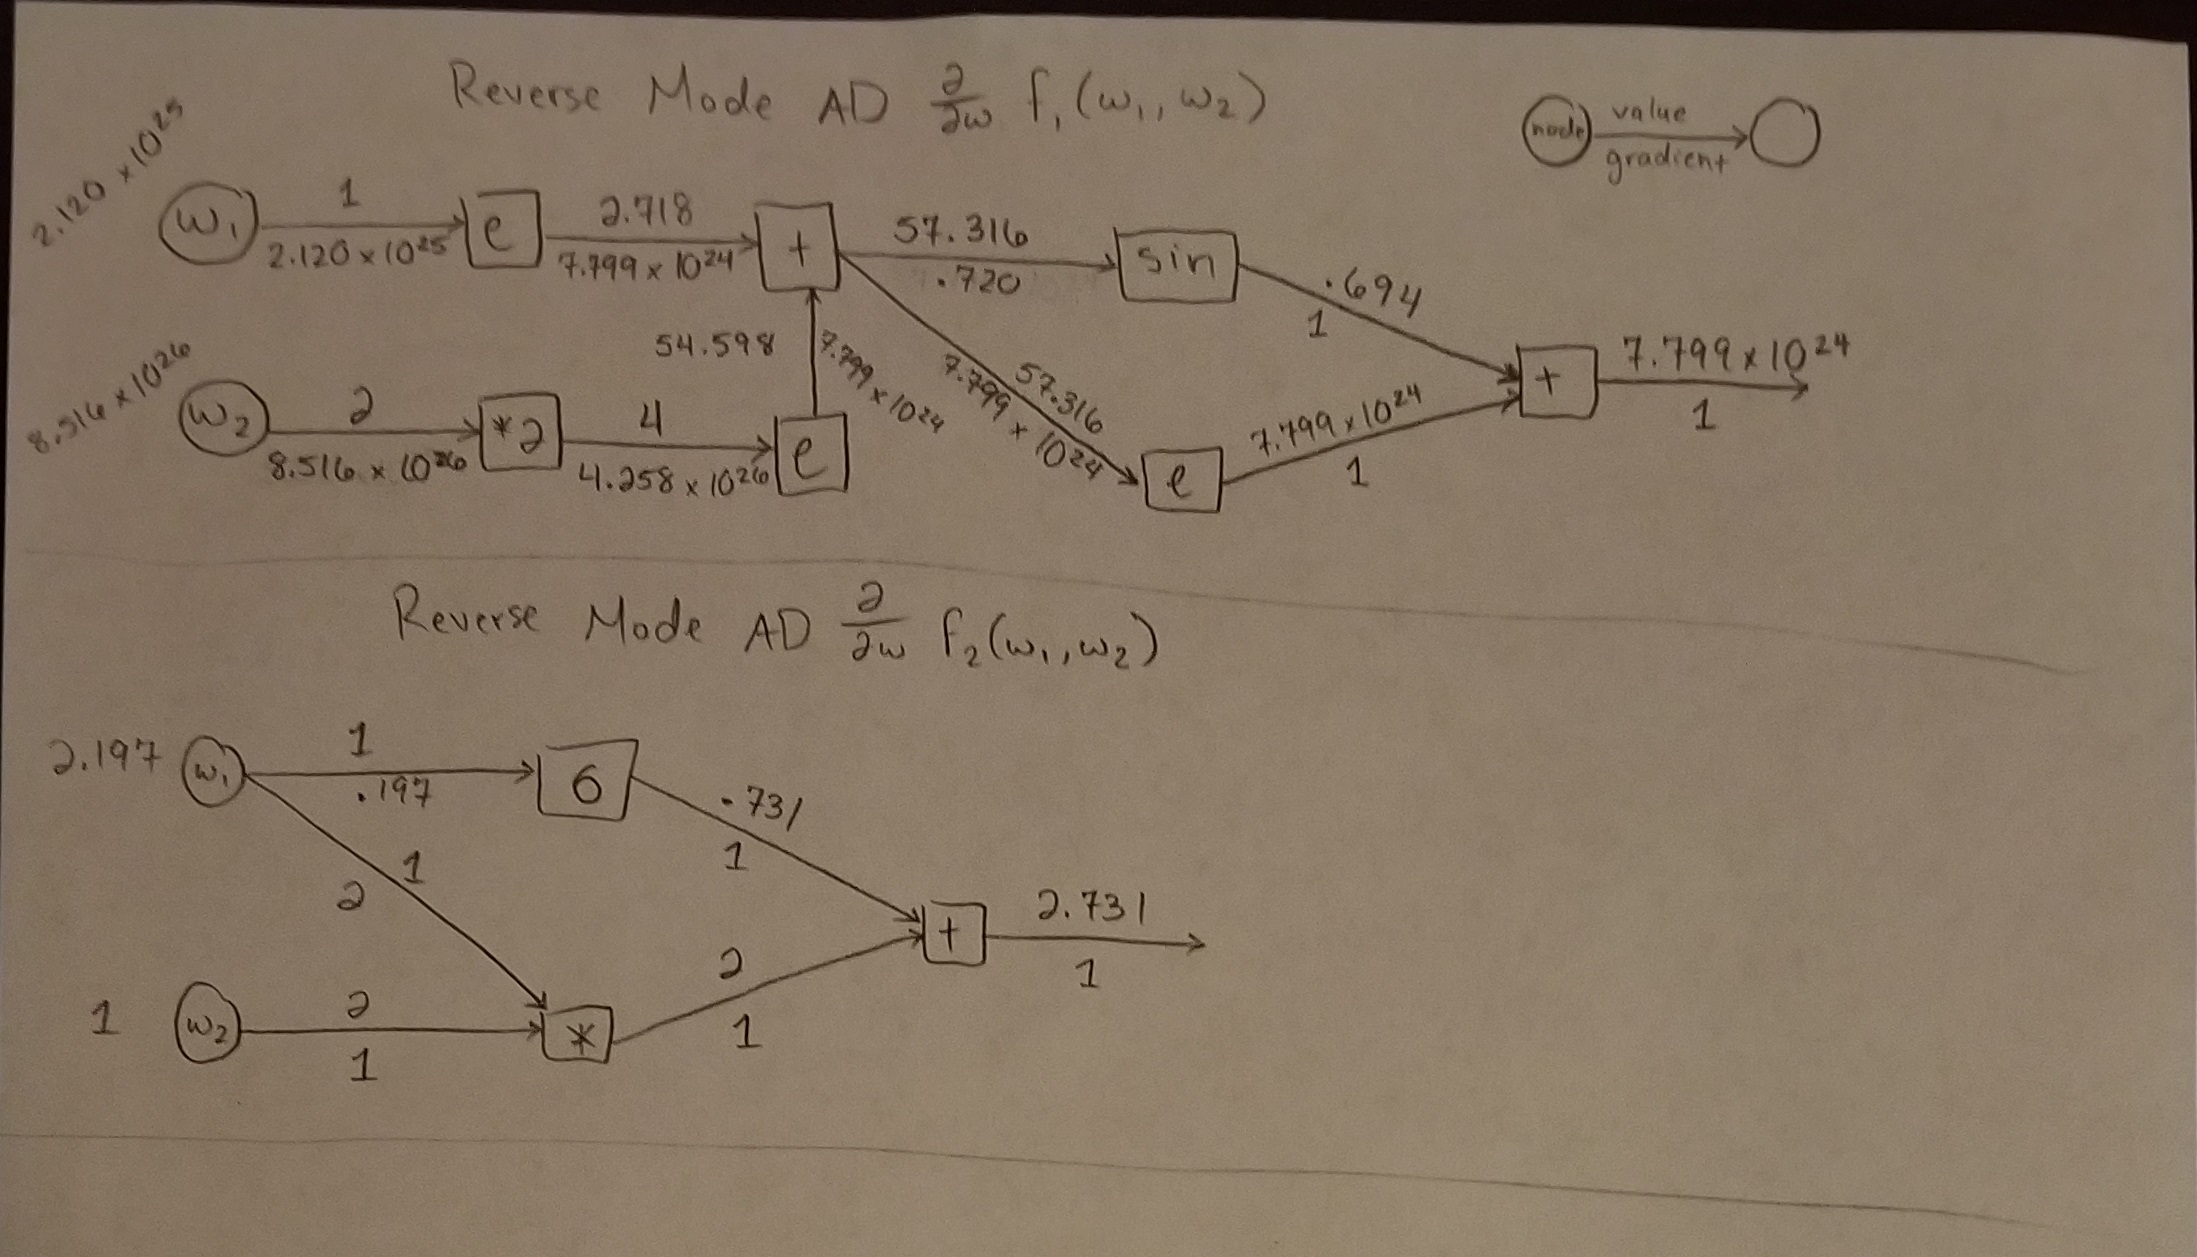
\includegraphics[scale=0.2]{5d.jpg}\\
	
	$J = \begin{bmatrix}
	2.120\times 10^{25} & 8.516\times 10^{26} \\
	2.197 & 1 \\[1ex] % <-- 1ex more space between rows of matrix
	\end{bmatrix}$\\\\
	\pagebreak
	
	$5(e).$\\
	
	This is torture. Yes.
	\pagebreak
	
\section{Directed Acyclic Graphs (DAG)}

$6.$\\

We want to show if a graph G is a DAG, it has a topological ordering.

Since G is a DAG, $\exists v_i \in V_G$ s.t. $v_i$ has no incoming cycle.

Now, let $V' = \emptyset$ be an empty queue of vertices.

Remove $v_i$ from $V_G$ and add it to $V'$ such that $V' = \{v_i\}$ and $G = G - v_i$.

G is still a DAG since removing a vertex does not add any edges to a graph.

Since G is still a DAG, $\exists v_j \in V_G$ s.t. $v_j$ has no incoming cycles.

Remove $v_j$ from $V_G$ and add it to $V'$ such that $V' = \{v_i, v_j\}$ and $G = G - v_j$.

G is still a DAG from the aforementioned logic.

We can repeat this process until $V_G = \emptyset$ and $\vert V'\vert = n$, indicating all vertices have been placed in this queue.

At this point, G is still a DAG because an empty set is a DAG by definition.

By removing the vertices of $V'$ in first-in-first-out order, we can easily retrieve a topological ordering of G because each vertex $v_m$ removed from the queue removes some edge $(v_m, v_k)$, allowing $v_k$ to be removed. This enforces an ordering of the vertices such that in order for a vertex $v_k$ to be removed, all vertices (e.g. $v_m$) directed into it must be removed first.

As such, if we enforce $m < k$, we have that for all edges $(v_m, v_k)$ we have $m < k$, which is the definition of a topological ordering.

$\therefore$ If G is a DAG, it has a topological ordering. $\qquad \qed$\\
\pagebreak

$7.$\\

We want to show that if G has a topological ordering, it is a DAG.

Since G has a topological ordering, we know that for all edges $(v_i, v_j) \in E$, we have $i < j$.

Assume some cycle C exists in G. Let $v_i$ be the vertex with the lowest number in the cycle.

The vertex directly preceding $v_i$, let us name it $v_j$, forms an edge $(v_j, v_i)$.

$\star$ Since $v_i$ is the lowest numbered vertex in the cycle, we know $i < j$.  

However, in order to enforce the topological ordering assumption, since $(v_j, v_i)$ exists, then $j$ must be less than $i$ ($j < i$).

This directly contradicts $\star$, so the cycle produces a contradiction of the topological ordering of G. As such, G must have no cycles (i.e. it is acyclic).

$\therefore$ G is a DAG. $\qquad \qed$

\end{document}
